\chapter[SVD with eigenvalues]{General case: SVD with eigenvalues}
\label{chap:general}
The general method for finding the \svdp \ demands finding the eigenvalues of either product matrix, $\W{x}$ or $\W{y}$. As we will see later, every matrix has a \svdl, and so having a robust general method guarantees that we can resolve every matrix into the component matrices.

%%
\section{Comparing two SVD strategies}
In the previous chapter we saw a quick and pedagogical method for composing an SVD. It clearly demonstrated the resolution of the domain and codomain and emphasized the elementary nature of the decomposition.

However, there are some shortcomings to the method: 
\begin{enumerate}
\item the essence of the singular values is obscured;
\item the method is not universal.
\end{enumerate}

While both methods rely upon augmented reduction, the general method also requires solving an eigensystem.

Table \eqref{tab:3:comparex} compares the simple method of the first chapter with the general method that we are about to explore. In this form the differences in strategy seem innocuous. In fact, the conception of the general method is comparable to the conception of the simple method. However, the general method requires solving an eigensystem. It is the resolution of the eigenvalues and eigenvectors for the product matrix that can make practical decompositions so daunting. 

\begin{table}[h]
\begin{center}
\begin{tabular}{l|cclll }
 & {\it construct} & {\it solve for} & {\it method} & {\it pros} & {\it cons} \\ \hline
 1 & $\X{}$, $\Y{}$ & $\Sigma$ & augmented reduction & easy & special cases \\[3pt]
 2 & $\X{}$, $\Sigma$ & $\Y{}$  & eigenvalue problem  & difficult & universal \\[3pt]\hline
\end{tabular}
\end{center}
\label{tab:3:comparex}
\caption{Comparing two strategies for the SVD. The easy method of chapter 1 is on top; the general method on the bottom.}
\end{table}%

%%
\section[The general method for SVD]{The general method for \svdl}

This chapter focuses on the most general method for computing an SVD. The requisite steps are elementary, but the combination of tasks can obscure the process. To minimize this \index{fog of computation}fog of computation the process is dissected and mounted in equation \eqref{eq:gen:flow} and tables \eqref{tab:3:} and \eqref{tab:3:input}. The tables are for reference.

%%
\begin{landscape}
\thispagestyle{empty}

\begin{equation}
  \begin{array}{ccccccccccccc}
  \A{}&\longrightarrow&\A{*}&\longrightarrow&\W{x}&\longrightarrow&\lambda\paren{\W{x}}&\longrightarrow&\lst{\sigma_{k}}&\longrightarrow&\sig{}\\
  &&&&\downarrow\\
  &&&&\lst{x_{k}}&\longrightarrow&\lst{x_{k}}^{\perp}&\longrightarrow&\X{}\\
  &&&&&&&&\downarrow\\
  &&&&&&&&\lst{y_{k}}&\longrightarrow&\lst{y_{k}}^{\perp}&\longrightarrow&\Y{}\\
  \end{array}
  \label{eq:gen:flow}
\end{equation}
Flow chart for a typical \svdl. This layout shows the simplicity of the underlying decomposition process. In general, it is the eigenvalue problem thats gives the SVD a reputation as being difficult.

To compute:
\begin{enumerate}
\item $\A{*}$, the Hermitian conjugate: compute $\overline{\A{}}^{\mathrm{T}}$;
\item $\W{x}$, the product matrix: compute $\prdm{*}$;
\item $\lambda(\W{x})$, the eigenvalue spectrum: solve $p(\lambda)=0$; i.e. find the $\rho$ nonzero roots of the characteristic polynomial;
\item $\lst{\sigma_{k}}, \  k=1,\rho$, the singular values of $\A{}$: arrange the nonzero products $\sqrt{\lambda}$ in descending order;
\item $\sig{}$, the matrix of singular values: embed the singular values along the diagonal of the sabot matrix of zeros;
\item $\lst{x_{k}},\  k=1,\rho$, the eigenvectors of $\W{x}$: find the null space vectors of $\W{x}-\lambda_{k}\I{n},\  k=1,\rho$;
\item $\lst{x_{k}}^{\perp},\  k=\rho+1,n$, the orthonormal perpendicular complement to $\lst{x_{k}}$: use the Gram-Schmidt process;
\item $\X{}$, the orthonormal basis matrix for the domain: arrange the vectors as $\X{}=\mat{c|c}{x_{k} & x^{\perp}_{j}}, \  k=1,\rho, \ j = \rho+1,n$;
\item $\lst{y_{k}},\  k=1,\rho$, the eigenvectors of $\W{y}$: compute $y_{k} = \sigma_{k}^{-1}\A{}x_{k},\  k=1,\rho;$
\item $\lst{y_{k}}^{\perp},\  k=\rho+1,m$, the orthonormal perpendicular complement to $\lst{y_{k}}$: use the Gram-Schmidt process;
\item $\Y{}$, the orthonormal basis matrix for the codomain: arrange the vectors as $\Y{}=\mat{c|c}{y_{k} & y^{\perp}_{j}}, \  k=1,\rho, \ j = \rho+1,m$.
\end{enumerate}

\clearpage
\thispagestyle{empty}

%%
\begin{table}[p]
\begin{center}
\begin{tabular}{lllcll}
 symbol & type & size & census & description & use \\\hline
 $\A{}$ & matrix & $\cmplx{\by{m}{n}}_{\rho}$ & 1 & target matrix  & input matrix \\
 $\A{*}$ & matrix & $\cmplx{\by{n}{m}}_{\rho}$ & 1 & Hermitian conjugate & intermediate matrix\\ 
 $\W{x}$ & matrix & $\cmplx{\by{n}{n}}_{\rho}$ & 1 & product matrix $\A{*}\A{}$ & intermediate matrix\\
 $\W{y}$ & matrix & $\cmplx{\by{m}{m}}_{\rho}$ & 1 & product matrix $\A{}\A{*}$ & intermediate matrix \\
 \ &&& \\
 $x_{k}$ & $n-$vectors & $\cmplx{\by{n}{1}}$ & $\rho$ & eigenvectors of $\W{x}$ & first $\rho$ columns of $\X{}$ \\
 $y_{k}$ & $m-$vectors & $\cmplx{\by{m}{1}}$ & $\rho$ & eigenvectors of $\W{y}$, $\paren{\sigma_{k}}^{-1}\A{}\X{}_{:,k}$ & first $\rho$ columns of $\Y{}$ \\
 $\paren{x_{k}}^{\perp}$ & $n-$vectors & $\cmplx{\by{n}{1}}$ & $n-\rho$ & orthogonal null space vector, domain & remaining $n-\rho$ columns of $\X{}$ \\
 $\paren{y_{k}}^{\perp}$ & $m-$vectors & $\cmplx{\by{m}{1}}$ & $m-\rho$ & orthogonal null space vector, codomain & remaining $m-\rho$ columns of $\Y{}$ \\
 \ &&& \\
 $\lambda_{k}$ & reals && $\rho$ & eigenvalues of the smaller of $\W{x}$, $\W{y}$ &intermediate product \\
 $\sigma_{k}$ & reals && $\rho$ & singular values $\sqrt{\lambda_{k}}$ & diagonal elements of $\sig{}$\\
 \ &&& \\
  $\ess{}$ & matrix & $\real{\by{\rho}{\rho}}_{\rho}$ & 1 & singular values matrix & intermediate matrix \\
  $\sig{}$ & matrix & $\real{\by{m}{n}}_{\rho}$ & 1 & $\sig{}$ matrix & output matrix \\
  $\X{}$ & matrix & $\cmplx{\by{n}{n}}_{n}$ & 1 & unitary domain matrix & output matrix \\
  $\Y{}$ & matrix & $\cmplx{\by{m}{m}}_{m}$ & 1 & unitary codomain & output matrix \\
[10pt]
\end{tabular}
\end{center}
\label{tab:3:personaedramatis}
\caption{Personae dramatis. This is a directory detailing the inputs, outputs and intermediary quantities used to find an SVD. The column vectors of the domain matrices $\X{}$ and $\Y{}$ are orthonormal.}
\end{table}

\end{landscape}
\clearpage
\break
%%
\begin{table}[h]
Given $\A{}\in\cmplx{\by{m}{n}}_{\rho}$, a matrix of rank $\rho$ with $m$ columns and $n$ rows, compute the \svdl \ $\A{}=\Y{}\,\Sigma\,\X{*}$ using these steps:\\[4pt]
\begin{enumerate}
\item Compute $\A{*}$, the conjugate of the transpose.\\[4pt]
\item Compute $\W{x}=\prdm{*}$.\\[4pt]
\item Solve for the $\rho$ ordered, nonzero eigenvalues $\lambda_{k}$ of $\W{x}$.\\[4pt]
\item Compute the $\rho$ singular values $\sigma_{k}=\sqrt{\lambda_{k}}, \ k=1,\rho$.\\[4pt]
\item Assemble $\sig{}$ the matrix of singular values. It is a sabot matrix of zeros with the $\rho$ singular values $\sigma_{k}$ on the diagonal in descending order.
\begin{equation}
  \Sigma = \underbrace{\mat{cccccccc}
  {
  \sigma_{1} & 0 & 0 & \cdots &&&& 0\\
  0 & \sigma_{2} & 0 & \dotsm &&&& 0\\
  0 & 0 & \ddots &&&&& \vdots \\
  \vdots & \vdots & & \sigma_{\rho} \\
   &  & & & 0  \\
   &  & & & & \ddots  \\
  0 & 0 &  & \cdots &&&& 0
  }}_{n \text{ columns}}
  \left. \phantom{\begin{array}{l}
  1\\
  1\\
  1\\
  1\\
  1\\
  1\\
  1\\
  1\\
  1
  \end{array}}\right\}
  m\text{ rows}.
\end{equation}
\item Solve for the $\rho$ eigenvectors $x_{k}$ of $\W{x}$.\\[4pt]
\item Compute $\tau_{x}=n-\rho$ orthonormal null space vectors for the perpendicular complement of the space spanned by these eigenvectors, $\lst{x}^{\perp}=\spn\lst{u_{1},\dots,u_{\tau_{x}}}$.\\[4pt]
\item Assemble the $\by{n}{n}$ matrix 
$\X{}=\mat{c|c|c|c|c|c}
{\hat{x}_{1} & \cdots & \hat{x}_{\rho} & \hat{u}_{1} & \dots & \hat{u}_{\tau_{x}}
}
$
for the domain.\\[4pt]
\item Solve for the $\rho$ vectors $y_{k}$, the orthonormal decomposition of $\rng{\A{}}$, using
\begin{equation}
  y_{k} = \paren{\sigma_{k}}^{-1}\A{} x_{k}.
\end{equation}
\item Compute $\tau_{y}=m-\rho$ null space vectors which are the  orthonormal perpendicular to the image space $\lst{y}^{\perp}=\spn\lst{v_{1},\dots,v_{\tau_{x}}}$ for the codomain.\\[4pt]
\item Assemble the $\by{m}{m}$ matrix 
$\Y{}=\mat{c|c|c|c|c|c}
{\hat{y}_{1} & \cdots & \hat{y}_{\rho} & \hat{v}_{1} & \dots & \hat{v}_{\tau_{y}}
}
$ for the codomain.\\[4pt]
\item Verify $\svd{*} = \A{}.$\\[6pt]
\end{enumerate}
\caption{Recipe for a \svdl. These are the basic tasks for the general purpose method to complete the full SVD. As with any recipe, there are variants. The simple method in the last chapter is one such variant. Consider these steps to be the most robust and general method. A hat over a vector implies normalization.}
\label{tab:3:input}
\end{table}

\clearpage
\break

\endinput
\section{The matrix of singular values}

In this volume we have, by fiat, restricted the singular values to being nonzero. This is a convention, by no means a theoretical necessity.


\begin{table}[htdp]
\begin{center}
\begin{tabular}{lccc|cc}
  $\A{}$ & $\sig{}$ & $\sig{T}$ & $\sig{(+)}$ & $\sig{}\sig{(+)}$ & $\sig{(+)}\sig{(+)}$\\
  $\cmplx{\bys{2}}_{2}$ &
  $\mat{cc}{\sigma_{1}&0\\0&\sigma_{2}}$ & 
  $\mat{cc}{\sigma_{1}&0\\0&\sigma_{2}}$ & 
  $\mat{cc}{\frac{1}{\sigma_{1}}&0\\0&\frac{1}{\sigma_{2}}}$ & $\itwo$ & 
  $\itwo$\\ 
  %%
  $\cmplx{\by{3}{2}}_{2}$ &
  $\mat{cc|c}{\sigma_{1}&0&0\\0&\sigma_{2}&0}$ & 
  $\mat{cc}{\sigma_{1}&0\\0&\sigma_{2}\\\hline 0&0}$ & 
  $\mat{cc}{\frac{1}{\sigma_{1}}&0\\0&\frac{1}{\sigma_{2}}\\[3pt]\hline 0&0}$ &
  $\itwo$ & 
  $\mat{cc|c}{1&0&0\\0&1&0}$\\
  %%
  $\cmplx{\by{2}{3}}_{1}$ &
  $\mat{c|c}{\sigma_{1}&0\\\hline0&0\\0&0}$ & 
  $\mat{c|cc}{\sigma_{1}&0&0\\\hline0&0&0}$ & 
  $\mat{c|cc}{\frac{1}{\sigma_{1}}&0&0\\[3pt]\hline0&0&0}$ &
  $\mat{c|cc}{1&0&0\\\hline0&0&0\\0&0&0}$ & 
  $\mat{c|c}{1&0\\\hline0&0}$ \\
  \ \\
\end{tabular}
\end{center}
\caption{Different forms for the $\sig{}$ matrix for three types of matrices. The matrices $\sig{}$ and $\sig{T}$ share the same diagonal; $\sig{T}$ and $\sig{(+)}$ share the same shape.}
\label{tab:sing}
\end{table}%

Stencils
truncated identity
\begin{equation}
  \begin{split}
    \sig{}\sig{(+)} &= \mat{c|c}{\I{m}&\zero\\\hline\zero&\zero} = \J{m}{\rho}, \\
    \sig{(+)}\sig{} &= \mat{c|c}{\I{n}&\zero\\\hline\zero&\zero} = \J{n}{\rho}.
  \end{split}
\end{equation}


\endinput
\section{The problem}
Apply the general method to the new target matrix
\begin{equation}
  \A{} = \mat{ccc}
  {
  0 & 3 & 0 \\
  1 & 2 & 2
  }
\end{equation}
and follow the steps in table \eqref{tab:3:input} to produce an SVD.\\

Diagnosis: the target matrix has rank 2 due to two independent rows. Therefore we can define the shapes of the component matrices as show in figure \eqref{fig:232}.
\begin{equation}
  \A{}\in\real{\by{2}{3}}_{2}.
\end{equation}
\begin{figure}[htbp] %  figure placement: here, top, bottom, or page
   \centering
%   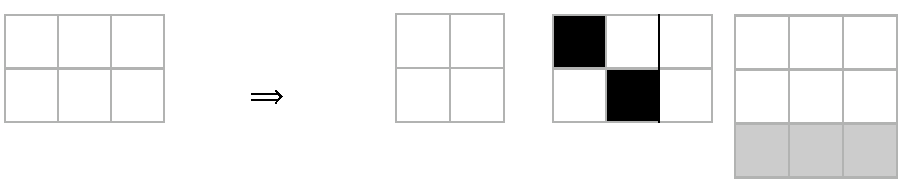
\includegraphics[ ]{pdf/general/svd_02_03_02} 
   \includegraphics[ ]{pdf/general/C232} 
   \caption[Shapes and dimensions]{The shapes and dimensions for the pending decomposition are determined by the shape of the target matrix. The rank tells us how many singular values we will find.}
   \label{fig:232}
\end{figure}
%%%

%%
\subsection{Compute the adjoint matrix $\A{T}$}
\begin{equation}
  \A{} = \mat{cc}
  {
  0 & 1 \\
  3 & 2 \\
  0 & 2
  }.
\end{equation}

%%
\subsection{Compute the product matrix $\W{x}$}
\begin{equation}
  \W{x}=\A{T}\A{}= \mat{ccc}{
 1 &  2 & 2 \\
 2 & 13 & 4 \\
 2 &  4 & 4}
\label{eq:problemgen:Wx}
\end{equation}

%%
\subsection{Find the eigenvalues of $\W{x}$}
We could solve this system for eigenvectors and eigenvalues. But the product matrix $\W{y}$ is a smaller and simpler system to resolve. So to reduce the amount of labor we will work with the other product matrix
\begin{equation}
  \W{y}=\A{}\,\A{T} =
\left[
\begin{array}{cc}
 9 & 6 \\
 6 & 9
\end{array}
\right].
\label{eq:problemgen:Wy}
\end{equation}
Details are in the appendix allowing a freedom to touch upon just the high notes. 

Start with a some simplification: remove common factors from the product matrix. To wit
\begin{equation}
  \W{y}=3\W{y}'.
  \label{eq:scale}
\end{equation}

To find the eigenvalues, find the the roots of the \index{characteristic polynomial} characteristic polynomial defined by
\begin{equation}
  p(\lambda) = \det \paren{\W{y}'-\lambda \I{2}} =
  \det \mat{cc}
  {
  3-\lambda & 2 \\
  2 & 3-\lambda
  }.
\end{equation}

In this instance we find
\begin{equation}
  p(\lambda) = \lambda^{2} - 6\lambda + 5
\end{equation}
which is easily factored. Extracting the roots to $p(\lambda) = 0$ yields $\lambda = \lst{5,1}$. Accounting for the scale factor in \eqref{eq:scale} we say the eigenvalue spectrum for the product matrix $\W{y}$ is given by
\begin{equation}
  \lambda = \lst{15, 3}
\end{equation}

\textbf{Caution:} Always arrange the eigenvalues in \textit{decreasing} magnitude.

%%
\subsection{Compute the singular values $\sigma_{k}$}
The singular values are the square root of the non-zero eigenvalues of the product matrices:
\begin{equation}
  \sigma = \sqrt{\lambda} = \lst{\sqrt{15},\sqrt{3}}.
\end{equation}

%%
\subsection{Build the $\sig{}$ matrix}
The $\sig{}$ matrix of singular values has the same dimensions are the target matrix. Populate the upper diagonal with singular values:
\begin{equation}
  \A{} = \mat{cc|c}
  {
  \sqrt{15} & 0 & 0 \\
  0 & \sqrt{3}  & 0
  }
\end{equation}

%%
\subsection{Find the eigenvectors of the product matrix $\W{x}$}
The eigenvalue problem for this example is this
\begin{equation}
  \W{x}\lambda_{k} = \lambda_{k} x_{k}, \quad k=\lst{1,\rho}.
  \label{eq:raw:ev}
\end{equation}
Here $x_{k}$ is the eigenvector of interest. Notice that we skip any cases where $\lambda=0$. Yes, this would provide null vectors, but they would not be an orthogonal set.

The canonical method for solving equation \eqref{eq:raw:ev} is to express it as a null space problem as they are easier to solve:
\begin{equation}
  \paren{\W{x} - \lambda_{k}\I{3}} = \zero, \quad k=\lst{1,\rho}.
\end{equation}
The two cases follow. Both will be solved by augmented reduction or EAR.
\begin{enumerate}
\item For $k=1$. The source matrix is given by
\begin{equation}
\W{x}-15\I{3} =
\left[
\begin{array}{rrr}
 -14 & 2 & 2 \\
 2 & -2 & 4 \\
 2 & 4 & -11
\end{array}
\right]. 
\end{equation}
The augmented system has this final form
\begin{multline}
\frac{1}{12}
\left[
\begin{array}{rrr}
 5  & 29 & 12 \\
 -1 & -7 & 0 \\
 6  & 30 & 12
\end{array}
\right]
\mat{rrr|ccc}
{
-14 & 2 & 2 & 1 & 0 & 0 \\
 2 & -2 & 4 & 0 & 1 & 0 \\
 2 & 4 &-11 & 0 & 0 & 1
}\\
=
\mat{crr|rrc}
{
1 & 0 & -\frac{1}{2}  &  \frac{5}{12} & \frac{29}{12} & 1 \\
0 & 1 & -\frac{5}{2}  & -\frac{1}{12} & -\frac{7}{12} & 0 \\[4pt]\hline\hline
0 & 0 & 0             &  \frac{1}{2}  & \frac{5}{2}   & 1
}.
\end{multline}
The double horizontal lines are drawn to accentuate the boundary of the null vectors. The row vectors of interest accompany the zero vectors on the bottom of the matrix on the right. In this case there is just one vector:
\begin{equation}
  x_{1}^{\mathrm{T}} = \mat{ccc}{1&5&2}
\end{equation}
After normalization, we have the first column in the domain matrix:
\begin{equation}
  \X{}_{*,1} = \hat{x}_{1} = \frac{1}{\sqrt{30}}\mat{c}{1\\5\\2}.
\end{equation}
\item For $k=2$
\begin{equation}
\W{x}-3\I{3} =
\left[
\begin{array}{rrr}
 -2 & 2 & 2 \\
 2 & 10 & 4 \\
 2 & 4 & 1
\end{array}
\right].
\end{equation}
The augmented system has this final form
\begin{multline}
\frac{1}{12}
\left[
\begin{array}{crc}
 1 & -5 & 12 \\
 1 &  1 & 0 \\
 6 & -6 & 12
\end{array}
\right]
\mat{rrr|ccc}
{
-2 & 2  & 2 & 1 & 0 & 0 \\
 2 & 10 & 4 & 0 & 1 & 0 \\
 2 & 4  & 1 & 0 & 0 & 1
}\\
=
\mat{ccr|crc}
{
1 & 0 & -\frac{1}{2}  &  \frac{1}{12} & -\frac{5}{12} & 1 \\
0 & 1 &  \frac{1}{2}  &  \frac{1}{12} &  \frac{1}{12} & 0 \\[4pt]\hline\hline
0 & 0 & 0             &  \frac{1}{2}  & -\frac{1}{2}  & 1
}.
\end{multline}
\end{enumerate}
With normalization, we have the second column in the domain matrix:
\begin{equation}
  \X{}_{*,2} = \hat{x}_{2} = \frac{1}{\sqrt{6}}\mat{r}{1\\-1\\2}.
\end{equation}

%%
\subsection{Construct a null space for the domain}
Part of the confusion about the decomposition comes from the wonderful fact that there are some permutations in the path and multiple ways to approach some steps.

Here there are different ways to construct this third vector and assure that it is perpendicular to the first two vectors. We choose to use the cross-product.

The cross-product between two \vvv s is computed as this
\begin{equation}
\mat{c}{x_{1}\\x_{2}\\x_{3}}
\times
\mat{c}{y_{1}\\y_{2}\\y_{3}}
=
\det
\mat{ccc}
{
\hat{i} & \hat{j} & \hat{k} \\
  x_{1} & x_{2}   & x_{3}   \\
  y_{1} & y_{2}   & y_{3}   \\
}
=
\mat{c}
{
x_{2}y_{3}-x_{3}y_{2} \\
x_{3}y_{1}-x_{1}y_{3} \\
x_{1}y_{2}-x_{2}y_{1} 
}.
\end{equation}
The solitary null space vector is
\begin{equation}
u_{1} = x_{1} \times x_{2} =
\mat{c}{1\\5\\2}
\times
\mat{r}{1\\-1\\2}
=
\mat{r}
{
 2 \\
 0 \\
-1 
}.
\end{equation}
Therefore
\begin{equation}
  \X{}_{*,3} =\hat{u}_{1} = \frac{1}{\sqrt{5}}
\mat{r}
{
 2 \\
 0 \\
-1 
}.
\end{equation}

%%
\subsection{Assemble the domain matrix $\X{}$}
The normalization busies the appearance:
\begin{equation}
  \X{} = 
\left[
\begin{array}{ cr >{\columncolor{ltgray}}r }
  \frac{1}{\sqrt{30}} & \frac{ 1}{\sqrt{6}} & \frac{-2}{\sqrt{5}}\\
  \frac{5}{\sqrt{30}} & \frac{-1}{\sqrt{6}} & 0 \\
  \frac{2}{\sqrt{30}} & \frac{ 2}{\sqrt{6}} & \frac{ 1}{\sqrt{5}}\\
\end{array}
\right].
\end{equation}

A useful alternative presentation of this matrix is to write it as column vectors as shown here:
\begin{equation}
\X{}=
  \mat{c|c|>{\columncolor{ltgray}}c}
  {
  \frac{1}{\sqrt{30}} \mat{r}{1\\5\\2} &
  \frac{1}{\sqrt{6}}  \mat{r}{1\\-1\\2} &
  \frac{1}{\sqrt{5}}  \mat{r}{2\\0\\1}
  }.
\end{equation}
This defeats the camouflage of the normalization constants and reminds us of the significance of the columns. It also simplifies the visual check of orthogonality.

%%
\subsection{Solve for $y_{k}$}
A vital formula needed for \index{jumping between domains}jumping between domain and codomain is this
\begin{equation}
  \A{}\X{}_{*,k} = \sigma_{k} \Y{}_{*,k}, \quad k=\lst{1,\rho}.
  \label{eq:vital}
\end{equation}
\begin{enumerate}
\item For $k=1$
For the first normalized vector in the codomain we need to solve
\begin{equation}
  \begin{split}
    \A{}\X{}_{*,1} &= \sigma_{1} \Y{}_{*,1}, \\
    \mat{ccc}
    {0 & 3 & 0\\
     1 & 2 & 2
    }
    \frac{1}{\sqrt{30}}
    \mat{c}{1\\5\\2}
    & = 
    \sqrt{15} \Y{}_{*,1}.
  \end{split}
\end{equation}
The solution is
\begin{equation}
  \Y{}_{*,1} = \frac{1}{\sqrt{2}}\mat{c}{1\\1}.
\end{equation}
\item For $k=2$
It may be tempting to guess the second and final vector in the codomain matrix; there are only two possible choices. But to do so would entail the risk of placing the minus sign in the wrong place. So much of the decomposition keeps the arbitrary signs in consistent use. After working out the details, the solution to
\begin{equation}
  \A{}\X{}_{*,2} = \sigma_{2} \Y{}_{*,2}
\end{equation}
is the vector
\begin{equation}
  \Y{}_{*,2} = \frac{1}{\sqrt{2}}\mat{r}{-1\\1}
\end{equation}
\end{enumerate}

%%
\subsection{Construct a null space for the codomain}
There is no null space for the codomain; the target matrix has full row rank.

%%
\subsection{Assemble the codomain matrix $\Y{}$}
The codomain matrix is given by
\begin{equation}
  \Y{} = \frac{1}{\sqrt{2}}
  \mat{rr}{1 & -1\\1 & 1}.
\end{equation}

%%
\subsection{Assemble and verify the decomposition}
The formal decomposition is
\begin{equation}
  \boxed{
  \begin{array}{ccccc}
    \A{} &=& \Y{} & \sig{} & \X{T}\\
  \mat{ccc}
  {
  0 & 3 & 0 \\
  1 & 2 & 2
  } 
  &=&
  \frac{1}{\sqrt{2}}
  \mat{rr}{1 & -1\\1 & 1}
  &
  \mat{cc|c}
  {
  \sqrt{15} & 0 & 0 \\
  0 & \sqrt{3}  & 0
  }
  &
  \mat{ crr }
 {\frac{1}{\sqrt{30}} & \frac{5}{\sqrt{30}} & \frac{2}{\sqrt{30}}\\
  \frac{ 1}{\sqrt{6}} & \frac{-1}{\sqrt{6}} & \frac{2}{\sqrt{6}} \\
  \rowcolor{ltgray}
  \frac{-2}{\sqrt{5}} & 0 & \frac{1}{\sqrt{5}}}\\[25pt]
  \end{array}.
  }
  \label{eq:general:ysxt}
\end{equation}

The best way to insure that all the signs on the entries in the domain matrices are correct is to verify the decomposition:
\begin{equation}
  \begin{split}
    \A{} &= \Y{}\paren{\sig{}\,\X{T}},\\
     &=
  \stwo
  \mat{rr}{1 & -1\\1 & 1}
  \paren{
  \stwo
  \mat{crc}
  {
  1 & 5  & 2 \\
  1 & -1 & 2
  }}, \\
  &=
  \mat{ccc}
  {
  0 & 3 & 0 \\
  1 & 2 & 2
  }.
  \end{split}
  \label{eq:gen:soln}
\end{equation}

\endinput
\section{Observations}
We have experienced the full process of \svdl, a series of basic steps. 

The options at many steps which allow easier decomposition confuse some practitioners. These options may be mistakenly juggled with path variations and the SVD process may seem hazy as a result. Keep these things straight in your mind:
\begin{enumerate}
\item Know what you are trying to do;
\subitem resolve the domain and codomain into orthonormal coordinate systems;
\subitem resolve the singular values.
\item Know the foundation issues;
\subitem the row and vector spaces may not fully span the host space;
\subitem the row and column vectors may be far from orthogonal.
\item Remember how to perform each step;
\subitem know how to find eigenvalues and eigenvectors using augmented reduction or other techniques;
\subitem know how to construct perpendicular spaces;
\subitem know how to construct and load the matrix of singular values.
\end{enumerate}

The examples here are pedagogic and illuminate the process and the machinations. Many useful matrices will quickly submit to a \svdl. Hence these theoretical examples are both helpful and useful. However, the decomposition is intractable for many matrices.

Eigenvector problems can be arbitrarily complex. The space may be incomplete and finding mother-daughter eigenvector pairs become a permutation problem which grows factorially. This can be a major impediment.

There are many excellent texts and on-line resources to help with the machinations of finding eigenvalues and constructing orthogonal complements. A survey is listed here:

\begin{table}[htdp]
\begin{center}
\boxed{
\begin{tabular}{lcccc}
  topic & Anton [] & Strang1 [] & Strang2 [] & Meyer [] \\\hline
  augmented reduction & pp. 10-20 & pp. 10-20 & pp. 10-20 & p. 118\\
  eigenvectors & pp. 10-20 & pp. 10-20 & pp. 10-20 & p. 489\\
  null spaces  & pp. 10-20 & pp. 10-20 & pp. 10-20 & p. 173
\end{tabular}
}
\end{center}
\label{default}
\caption{Resources to help with facets of the \svdl.}
\end{table}


\endinput
\section{Exercises}
\begin{enumerate}
\item Consider the SVD given for $\Arrr{2}{2}{2}$:
\begin{equation*}
  \svdax{T} = 
  \mat{c|c}{y_{11} & y_{12} \\ y_{21} & y_{22}}
  \mat{cc}{\sigma_{1} & 0 \\ 0 & \sigma_{1}}
  \mat{cc}{x_{11} & x_{12} \\\hline x_{21} & x_{22}}.
\end{equation*}
Show by direct computation of the product that
\begin{equation*}
\begin{split}
  \A{} 
  &= \mat{cc}{
  \sigma_{1} x_{11} y_{11} + \sigma_{2} x_{12} y_{12} & \sigma_{1} x_{21} y_{11} + \sigma_{2} x_{22} y_{12} \\
  \sigma_{1} x_{11} y_{12} + \sigma_{2} x_{12} y_{22} & \sigma_{1} x_{21} y_{12} + \sigma_{2} x_{22} y_{22} } \\
  &= \sigma_{1} \mat{cc}{
  y_{11} \mat{cc}{x_{11} & x_{21}} \\
  y_{12} \mat{cc}{x_{11} & x_{21}}}
  + \sigma_{2} \mat{cc}{
  y_{21} \mat{cc}{x_{12} & x_{22}} \\
  y_{22} \mat{cc}{x_{12} & x_{22}}} \\
  &= \sigma_{1} y_{1}x_{1}^{T} + \sigma_{2} y_{2}x_{2}^{T}.
\end{split}
\end{equation*}
\item
\item
\end{enumerate}


\endinput

\endinput